\subsection{Dataset Curation}

Our evaluation dataset is derived from a proprietary, human-authored Obsidian knowledge base of mathematical problem-solving notes (455 notes, 1596 bidirectional links). Unlike standard (problem, proof) datasets, each note contains the author's reasoning process: problem reinterpretation, technique identification, difficulty progression, and connections to related problems. The link structure encodes an explicit relational graph where a few high-level strategies (hub nodes) connect to many specific problems (leaf nodes), following a power-law degree distribution (Figure~\ref{fig:tiers}).

Raw notes require curation because one note may contain multiple problems (original, strengthened, generalized), and edges are at note level rather than problem level. Our pipeline has four steps: (1)~extract individual problem statements from each note, (2)~rebuild connections at the problem level (inherited edges from note-level links, internal edges from within-note progression), (3)~formalize each problem as a Lean~4 theorem statement with \texttt{sorry} and verify compilation, (4)~classify nodes into problem nodes (formalizable) and technique nodes (pure strategy descriptions). The 34 hub nodes (degree $\geq$10, 7\% of total) serve as ground-truth strategy labels for evaluation.

\begin{figure}[h]
  \centering
  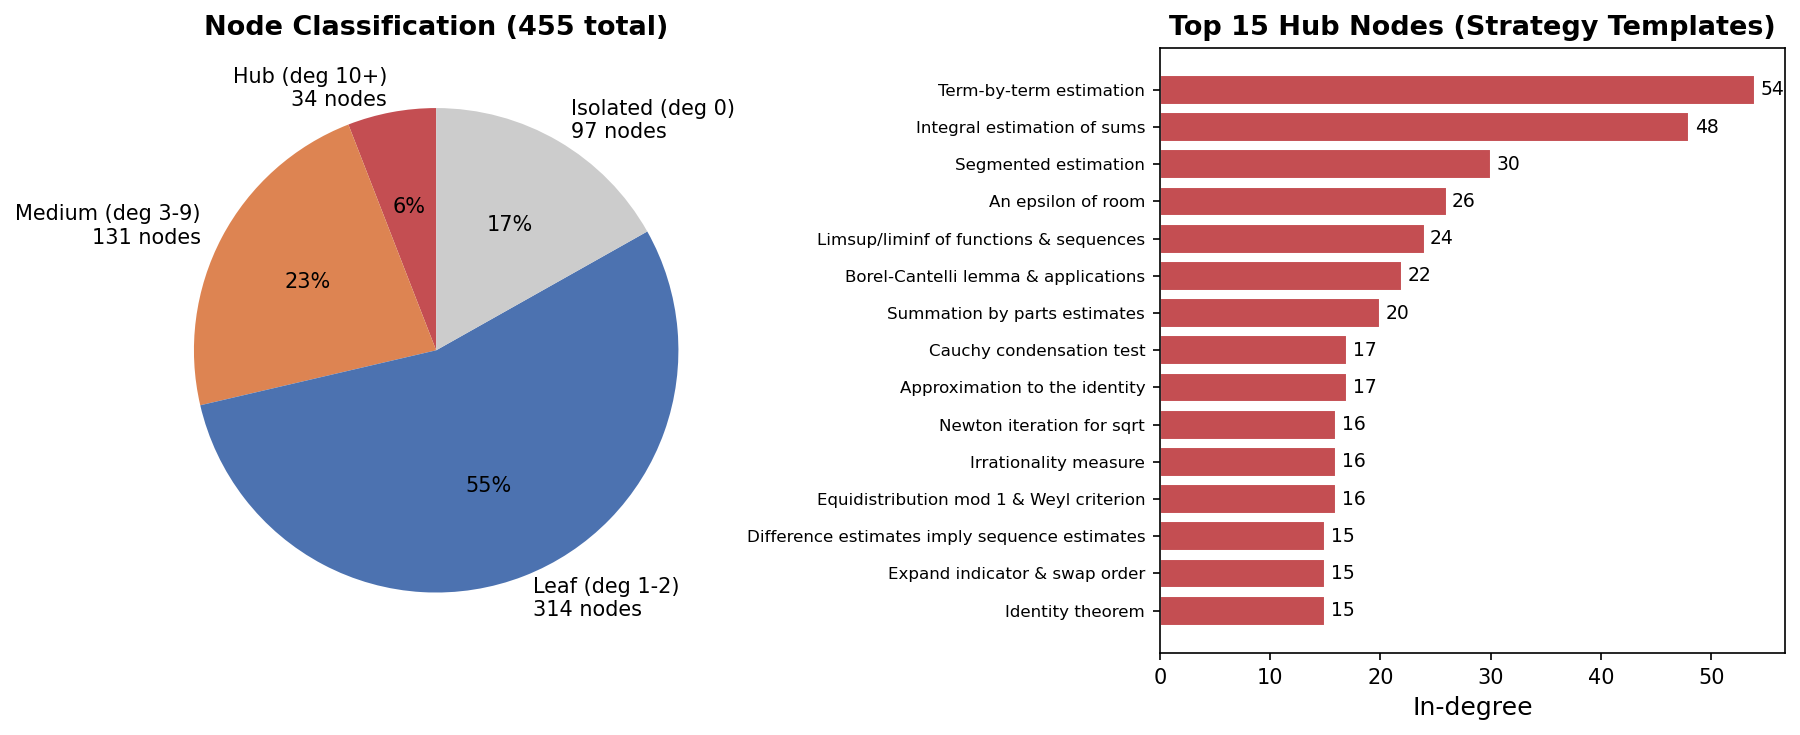
\includegraphics[width=\linewidth]{figures/tier-breakdown}
  \caption{Left: node classification by in-degree tier (455 total). Right: top 15 hub nodes representing reusable strategy templates.}
  \label{fig:tiers}
\end{figure}

\subsection{Evaluation 1: Prover Effectiveness}

We compare our structured workflow (plan--implement--replan with mechanization separation) against free agents (same model, same Lean checker MCP tool, no structured workflow). Baselines include Claude Code, OpenCode, and dedicated provers such as ReProver and Lean Copilot. Metrics: (1)~\textbf{Pass@k}---does the agent produce a sorry-free proof? (2)~\textbf{Iteration count}---how many LLM $\leftrightarrow$ Lean checker rounds? (3)~\textbf{Error type}---mechanization (wrong API name, syntax, type mismatch) versus mathematical (wrong strategy, dead-end decomposition).

\subsection{Evaluation 2: Knowledge Extraction Quality}

We evaluate whether the digest agent extracts deep, transferable knowledge or shallow summaries. The baseline is prompt-based summarization (``summarize the key ideas of this proof''). The setup: given a problem and its proof trace, the agent extracts lessons, which are then compared against ground-truth edges from the knowledge graph via semantic matching. Metrics: \textbf{precision} (of the connections the digest claims, how many match ground-truth edges?) and \textbf{recall} (of the ground-truth edges, how many does the digest recover?), weighted toward hub connections since recovering a link to a high-degree strategy template is more valuable than recovering a leaf-to-leaf connection.
